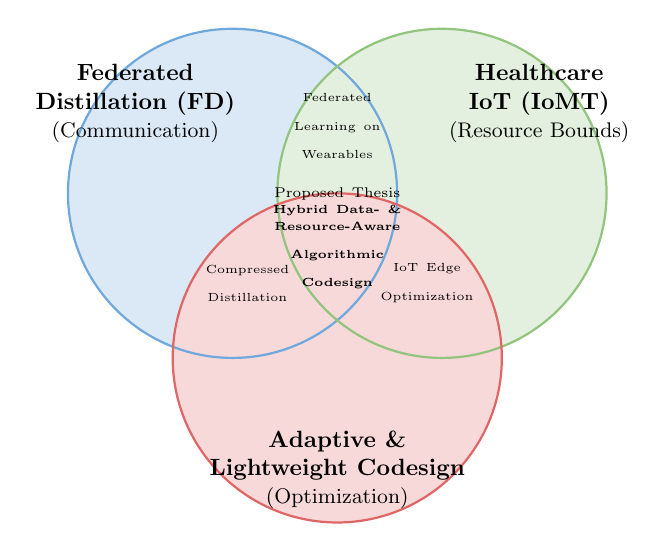
\begin{tikzpicture}[scale=0.95, every node/.style={scale=0.85}, line join=round, line cap=round]
    % Define custom harmonious pastel colors
    \definecolor{colorfd}{RGB}{111,168,220}   % Soft blue
    \definecolor{coloriot}{RGB}{147,196,125}  % Soft green
    \definecolor{colorcodesign}{RGB}{224,102,102} % Soft red/rose

    % Fills with high transparency for neat overlap mixing
    \fill[colorfd!25] (0,0) circle (2.2cm);
    \fill[coloriot!25] (2.8,0) circle (2.2cm);
    \fill[colorcodesign!25] (1.4,-2.2) circle (2.2cm);

    % Draw thin professional borders
    \draw[colorfd, thick] (0,0) circle (2.2cm);
    \draw[coloriot, thick] (2.8,0) circle (2.2cm);
    \draw[colorcodesign, thick] (1.4,-2.2) circle (2.2cm);

    % Circle Labels
    \node at (-1.3, 1.2) [align=center] {\textbf{Federated}\\\textbf{Distillation (FD)}\\\small(Communication)};
    \node at (4.1, 1.2) [align=center] {\textbf{Healthcare}\\\textbf{IoT (IoMT)}\\\small(Resource Bounds)};
    \node at (1.4, -3.7) [align=center] {\textbf{Adaptive \&}\\\textbf{Lightweight Codesign}\\\small(Optimization)};

    % Double Intersections (Peripheral domains in literature)
    \node at (1.4, 0.9) [align=center, text width=2cm] {\tiny Federated Learning on Wearables};
    \node at (0.2, -1.2) [align=center, text width=1.5cm] {\tiny Compressed Distillation};
    \node at (2.6, -1.2) [align=center, text width=1.5cm] {\tiny IoT Edge Optimization};

    % Core Triple Intersection (Your Research Question sits here!)
    \node at (1.4, -0.6) [align=center, text width=2.4cm] {
        \fontsize{6.5pt}{8pt}\selectfont
        \keyterm{Proposed Thesis}\\
        \fontsize{5.5pt}{7pt}\selectfont
        \textbf{Hybrid Data- \&}\\
        \textbf{Resource-Aware}\\
        \textbf{Algorithmic Codesign}
    };
\end{tikzpicture}
